\begin{frame}
  \frametitle{Interaction implies heterogeneity}
  The interaction index measures the contribution of the interaction terms:

  \begin{itemize}
    \item \(f(x_1, x_2) = x_1^2 + \log(x_2) + \alpha x_1x_2^3\)
    \item \(\alpha = 0.1 \rightarrow\) low interaction index \(\rightarrow\) high fidelity
    \item \(\alpha = 100 \rightarrow\) high interaction index \(\rightarrow\) low fidelity
    \end{itemize}
  \noindent\makebox[\linewidth]{\rule{\paperwidth}{0.4pt}}
  But it does not say how the interaction terms influence the feature effect plots
\end{frame}

\begin{frame}
  \frametitle{Example}
  \begin{figure}
    \centering
    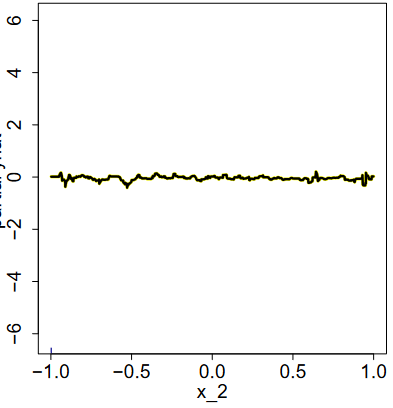
\includegraphics[width=1\textwidth]{pdp}
    \caption{PDP plot, taken from }
  \end{figure}
\end{frame}
